\documentclass[acmtog]{acmart}

\begin{document}

%%
%% The "title" command has an optional parameter,
%% allowing the author to define a "short title" to be used in page headers.
\title{Poster Abstract: Time series forecasting of European Energy Market
}

%%
%% The "author" command and its associated commands are used to define
%% the authors and their affiliations.
%% Of note is the shared affiliation of the first two authors, and the
%% "authornote" and "authornotemark" commands
%% used to denote shared contribution to the research.
\author{Hun Rim}
% \authornote{}
\email{rimh@usi.ch}
\author{Juraj Kardos}
\authornotemark[1]
\email{xxx@usi.ch}
\affiliation{%
  \institution{Università della Svizzera italiana}
  \streetaddress{Via Giuseppe Buffi 13}
  \city{Lugano}
  \state{Ticino}
  \country{Switzerland}
  \postcode{6900}
}

%%
%% The abstract is a short summary of the work to be presented in the
%% article.
\begin{abstract}
Due to climate change, the EU is transitioning towards renewable energy, aiming to increase its share in gross energy consumption to 42.5\% by 2030 from the current 23\%. However, the intermittent and seasonal nature of renewable energy sources presents challenges in predicting their production capacity. In this dynamic and ever-evolving landscape of the energy market, the ability to accurately forecast the evolution of renewable energy’s stake in the market is a critical component in the decision making process of policy makers, and market participants alike. This project aims to explore and evaluate the performance of well-established forecasting methods in anticipating the trends of individual renewable energy components, ultimately contributing to the fostering of a balanced, sustainable, and reliable energy market in the EU. \\

The primary focus of our framework is to assess auto-regressive forecasting methods, which leverage chronological data intervals to capture temporal dependencies from market history, thus ensuring accurate forecasting. However, instead of evaluating the model purely reliant on auto-regression, we examine more intricate models which extend to incorporate moving-average, exploit seasonality of time series data, or those utilising the correlation with exogenous variables. Furthermore, To get a better understanding of not only accuracy, but precision of the models, short-term forecasts are made iteratively to provide a bigger pool of model performance samples. All model’s performance in forecasting the individual energy components are evaluated by measuring and visualising the  Root Mean Square Percentage Error between forecast result and the test data. \\



\end{abstract}

\keywords{Time series, Forecasting, Energy Market, Predictive analytics, ARIMA}
\maketitle

\section{Introduction}

Like a staple good, we have steady demand for energy in our daily lives unlike luxury goods. When visualized, monthly energy demand reveals distinct patterns, with cyclical peaks occurring during winter and lows in summer, notably in July and August. These observations highlight Europe's heightened energy consumption in colder seasons and highlight the data's \textbf{seasonality}, suggesting the possibility of translating these patterns into mathematical models for forecasting future values.\\ 

\subsection{ARIMA}
ARIMA model is one of the most widely used statistical forecasting model, and it is the center of our evaluation. It is a generalized version of AutoRegressive Moving-Average (ARMA) model and difference between the two models is their ability to handle non-stationary data. Stationarity indicates constancy of statistical property of a dataset such as variance, or mean over time. When data is stationary, it guarantees the stability of underlying patterns in the dataset, and eradicates the concern of the pattern being a result of random fluctuation. ARIMA model is capable of adjusting the data to provide this stability unlike ARMA. \\

Autoregression is a technique used in time series analysis that assumes temporal trend between the values in the dataset, and uncover a function of order \textit{p}. In the auto-regression model, the variable regresses against itself. Put simply, the current value is calculated using past values, by estimating the influence of these past values (${\phi_1, \phi_2, ... \phi_p}$) on the present value. However, even if we assume the general trend is captured perfectly, there are inconsistent white-noise in the data which are not replicable. Hence, ARIMA model improves the accuracy by replicating these small bumps in the data through factoring in the anomalies in the recent data. All these factors are combined to formularize ARIMA model as the following:

\begin{displaymath}
    \hat{L}_N^{(d)} = C + \sum_{i=1}^{p} \psi_i L_{N - i}^{(d)} + \sum_{j=1}^{q}\varphi_j\epsilon_{N-j} + \epsilon_{N}
\end{displaymath}

\subsection{Seasonality}

As mentioned before, there is a clear seasonality in EU energy market and it would be preferable to incorporate this. There is a ARIMA's variation called S(easonal)ARIMA which extends to look into same interval in previous seasons. When the duration of the season is given, the SARIMA model breaks the data down into seasons and study recurring patterns in those segments. Hence, the estimation of the current value in SARIMA model is carried out as the following:

\begin{displaymath}
    SARIMA = \hat{L}_N^{(d)} + \sum_{i=1}^{P}\Phi_i L_{N - im}^{D} + \sum_{j=1}^{Q}\Theta_j \epsilon_{N - jm}  
\end{displaymath} 

\subsection{Deep-Learning}
Along with predictive statistics, deep learning is frequently used in forecasting. Especially, deep-learning using Recurrent-Neural-Network (RNN) is very popular with time series forecasting. As the name suggests, RNN has a property of repeating the process of aggregation and activation unlike normal neural networks. This regression like property of RNN makes it very effective when building a forecasting model, and it would be interesting to evaluate it's performance in comparison to conventional statistical methods. Hence, RNN forecasting method is also in progress of evaluation. \\

\section{Method ${\&}$ Material}

\subsection{Procedure}
\begin{itemize}
    \item ${(p, d, q)}$ order calculation.
    
There are 2 common methods in calculating the ${(p, d, q)}$ values. First method is calculating the ${d}$ value through differencing and \textit{Augumented Dickey-Fuller test}, then finding the order of autoregression (${p}$) through studying temporal correlation using ACF and PACF. Another method is implementing a grid search algorithm which finds the minimum Akaike Information Criterion (AIC) value by trying different combinations of ${(p, d, q)}$ within a given range. Naturally, first method is more efficient whereas the second method is computationally inefficient but simple to implement. However, as computational inefficiency problem is becoming negligent due to the significant enhancement of computational power, we decided to utilize \textit{auto\_arima()} function of \textbf{Python}. Which is a built-in grid search algorithm from \textit{pmdarima} library. \\

However, in certain cases the ${p, d, q}$ (order) calculated using library function doesn't return the global AIC minima due to the efficient library implementation. Hence, we had to build our own grid search algorithm which found the minima amongst all combinations in case the returned order was unsatisfactory (i.e. (0, 0, 0)). As a result, in exchange for negligent increase in execution time, the result of the grid search became much more feasible. \\

\item Train Test Split

To train and measure the performance of the forecasting model, we split our data into two parts, training set and test set. We train the model using 60\% of our data and assign the remaining 40\% as test data set to compare it with the forecast. \\

\item Training \& Forecasting

For training of the model, we use Python functions from ${statsmodels}$ library. The calculated order and seasonal order are passed to the trainer functions along with the train data set. Each model has respective trainer function provided from the ${statsmodels}$ library (${ARIMA(), SARIMAX()}$) and are configured accordingly with required training data, order of auto-regression, differencing, and moving-average. Finally, the model is fitted to the passed training data. \\

Then the trained model is used to make a forecast using the model class's ${Predict()}$ function from the starting month to the ending month of our designation. Which in our case has an interval of 3 months.\\

\item Rolling Horizon Approach

The forecast relies on historical values for estimation, which limits the model's ability to capture incoming trends, resulting in decrease of accuracy as the forecast window increases. To avoid this issue, forecasts are made at quarterly intervals. This approach is particularly necessary because the ARIMA model cannot incorporate new forecast errors into its formula, creating a need for iterative recalculation when the training set is updated. Therefore, we adopt the rolling horizon approach, where after each forecast, the training dataset is expanded by one month, and the model is re-trained before forecasting the future values of subsequent three months. By implementing the rolling horizon approach, the model becomes capable of incorporating real-time updates, mimics continuous learning, and avoids forecasting biases.\\

\item Analysis

Measuring the performance of forecasting method requires specific metric as our interest is in the relative error between predicted and actual values. Hence, we are using Root-Mean-Squared-Percentage-Error (RMSPE) as the metric for the performance measurement. Similar to Root-Mean-Squared-Error (RMSE), lower values in RMSPE indicate better performance. RMSPE measures the average percentage deviation between predicted and actual values, providing a standardized measure of prediction accuracy that is independent of the scale of the data. The data used for forecasting is not normalized and individual energy components have radically different scale. RMSE is capable of highlighting the difference in model's performance in individual energy components, however, it is not suitable for evaluating how accurate our forecast is, or for showcasing the overall performance. Hence, the RMSPE value provides better insight in evaluating forecasting models. \\

RMSPE value can be derived as the follwing:
\begin{displaymath}
\text{RMSPE} = \sqrt{\frac{1}{n} \sum_{i=1}^{n} \left( \frac{(Y_i - \hat{Y}_i)}{Y_i} \right)^2} \times 100
\end{displaymath} \\

\item Exogenous Variable

The EU power sector, just like any other power sector, experiences volatility due to exogenous factors such as the climate or the economy. Hence, the framework evaluates another ARIMA extension called SARIMAX (SARIMA + eXogenous variables) which also is capable of accounting for fluctuations due to the exogenous factors. In this model the exogenous variable which has influence on the European power sector such as the economic or climate indicators are passed to the appropriate time frame. Every data point in time series dataset needs corresponding exogenous variable, and all of them are gathered as a list and passed to SARIMAX function. When forecasting the market movements, the model can reflect on the previous values with similar indicator behaviors from the exogenous variable list to account for the influence of external factors, providing a more comprehensive and accurate forecast.
\end{itemize}

\subsection{Data}

The dataset consists of monthly energy components contributing to the energy balance on the supply and demand side as time series data. The data are published by the national authorities of European countries (usually the transmission system operators or the statistical office) and are collected on the level of the high-voltage transmission grid. The focus of this study is put on the key energy components or the components with the high level of variability, particularly electricity demand, and renewable energy generation such as wind, PV or hydro.  Electricity demand  is crucial for understanding how much power the system needs to meet consumer needs. Demand can vary significantly based on seasonal factors (heating/cooling), economic activity, and population growth. The increasing penetration of renewables significantly impacts supply dynamics. Understanding the variability of wind and solar generation, as well as the dispatchability (controllable generation) of hydro, is critical for managing grid integration challenges and optimizing renewable energy utilization. Data from the January of 2016 onwards is chosen as this period coincides with a significant ramp-up of renewable energy deployment across Europe. Analyzing data from this period allows us to track the evolving energy mix and its impact on power market dynamics. \\

\section{Result \& Discussion}

\subsection{Result Table}
\begin{figure}[hbt!]
    \centering
    \resizebox{0.45\textwidth}{!}{
    \begin{tabular}{cccccc}
    \toprule
    Date & Mean & SARIMA & ARIMA & S-Order & A-Order \\
    \midrule
    2023-03-01 & 35980 & 8.20 & 93.98 & (1,0,0)X(2,0,2,12) & (5,0,0)  \\
    2023-04-01 & 32624 & 4.73 & 2.83 & (1,0,1)X(5,0,0,12) & (5,0,0)  \\
    2023-05-01 & 31530 & 1.96 & 82.48 & (3,0,0)X(0,0,2,12) & (5,0,0)  \\
    2023-06-01 & 31202 & 9.86 & 48.31 & (1,0,0)X(2,0,2,12) & (5,0,0) \\
    2023-07-01 & 31312 & 13.93 & 1.08 & (1,0,0)X(2,0,1,12) & (5,0,0) \\
    2023-08-01 & 31660 & 11.80 & 2.83 & (1,0,1)X(2,0,1,12) & (5,0,0) \\
    \bottomrule
    \end{tabular}}
    \caption{Forecast result of power demand in France}
    \label{fig:forecast_result}
\end{figure}

The Figure (~\ref{fig:forecast_result}) is a showcase of the framework evaluating the performance of forecast models using rolling horizon approach through RMSPE metrics, where SARIMA and ARIMA column contains the RMSPE of the forecast against the test value. The table indicates SARIMA model's RMSPE is evenly distributed between approximately 2 to 14, and ARIMA model's RMSPE ranges from approximately 1 to 94 with higher concentration on the lower end (below 3). As mentioned before, lower RMSPE indicates higher performance of the model. Which means SARIMA model in general performs better than ARIMA model, and is more stable in terms of both accuracy and precision. Furthermore, SARIMA-Order (S-Order) seems to be constantly updated, where as ARIMA-Order (A-order) remains constant. This could be interpreted as SARIMA model better reflects the change in trend and seasonality with the consideration of ${seasonality}$ factor, in comparison to the ARIMA model. \\

\subsection{Visualization}

\begin{figure}[htb!]
    \centering
    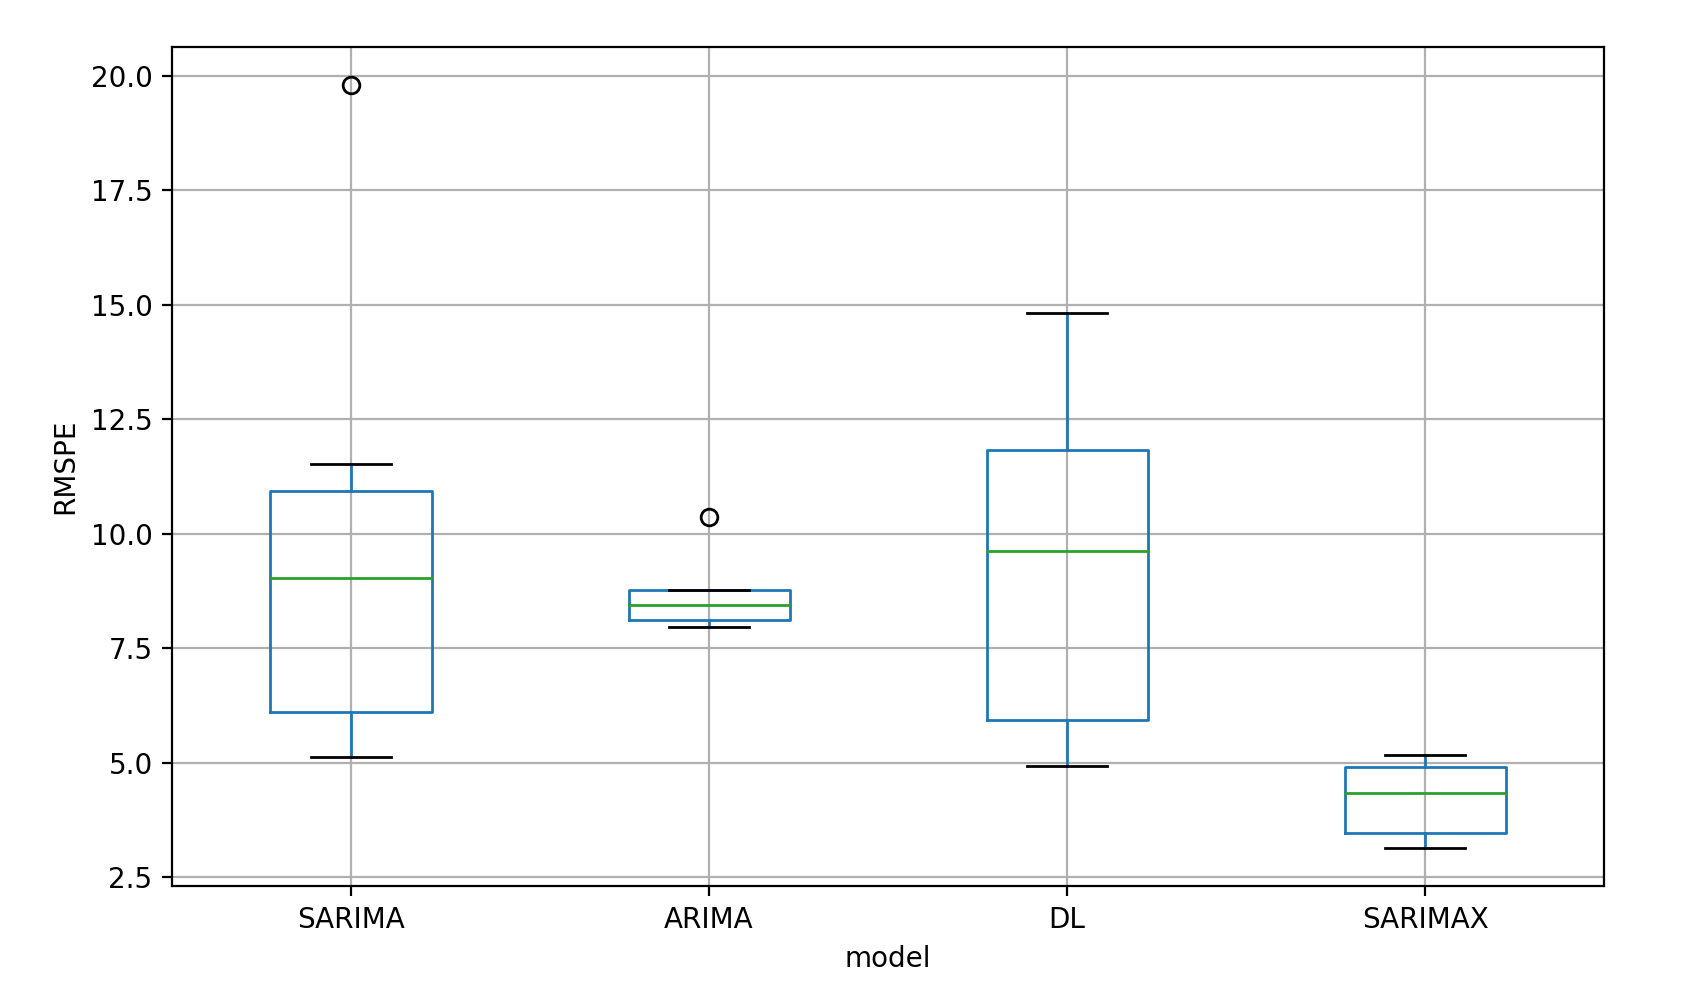
\includegraphics[width=0.4\textwidth]{figures/Figure_3.png}
    \caption{France energy demand forecast performance visualization}
    \label{fig:demand_performance_forecast} % Tag for referencing
\end{figure}

Figure (~\ref{fig:demand_performance_forecast}) above is the visualization of the SARIMA and ARIMA's performance through box-plotting the RMSPE values. This visualization is particularly useful when we are viewing larger scale of performance data from different energy sources and different countries as we don't have to individually read all tables. It displays how accurate the majority of the forecast's are while denoting the spread of the RMSPE values, and the anomalies in the data that are far off from general performance. Hence, enabling simple visual analysis of the result while making the anomalies easier to spot. The box-plots indicate SARIMA model was approximately 15\% off at worst case, and almost completely accurate in the best cases with median of approxitely below 10\%. Whereas ARIMA model has similar result to SARIMA model in case of best case scenario, while its median and worst case is far worse than that of the SARIMA. It is quite obvious that forecast error of this scale is not originiating from residual factors, and it is more likely to be due to the trend. \\


\begin{figure}[htb!]
    \centering
    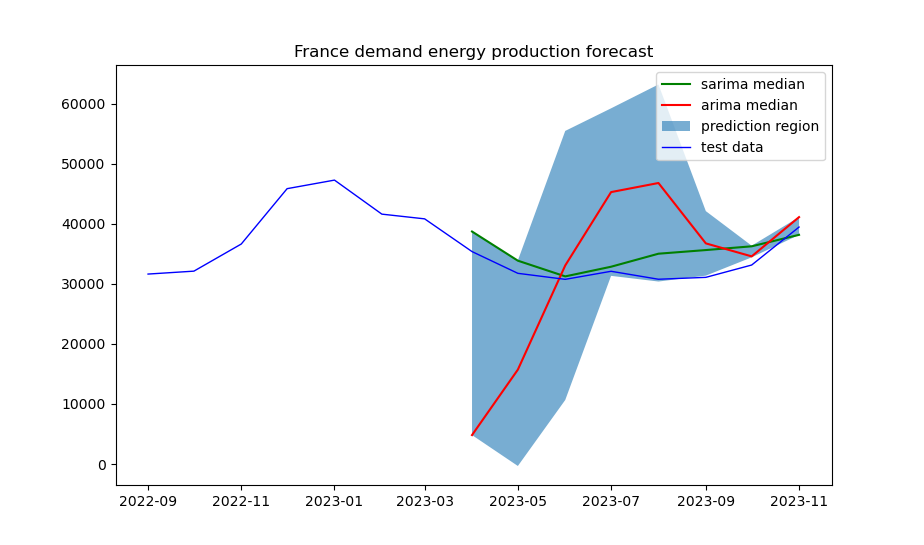
\includegraphics[width=0.4\textwidth]{figures/Figure_2.png}
    \caption{France energy demand forecast}
    \label{fig:demand_forecast} % Tag for referencing
\end{figure}

Figure (~\ref{fig:demand_forecast}) displays the forecast made from SARIMA and ARIMA model against the actual values. The shaded region is calculated from finding the maximum and the minimum of a merged forecast results. The green function is generated from the median value of the SARIMA forecasts, and the red function is the function generated from the median value of the ARIMA forecasts. As shown both on figure (~\ref{fig:forecast_result}) and figure (~\ref{fig:demand_performance_forecast}), ARIMA model performs quite poorly in most of the time excluding the last 2 months while SARIMA model performs consistently well over time. However, this is quite a rare case. \\

\begin{figure}[htb!]
    \centering
    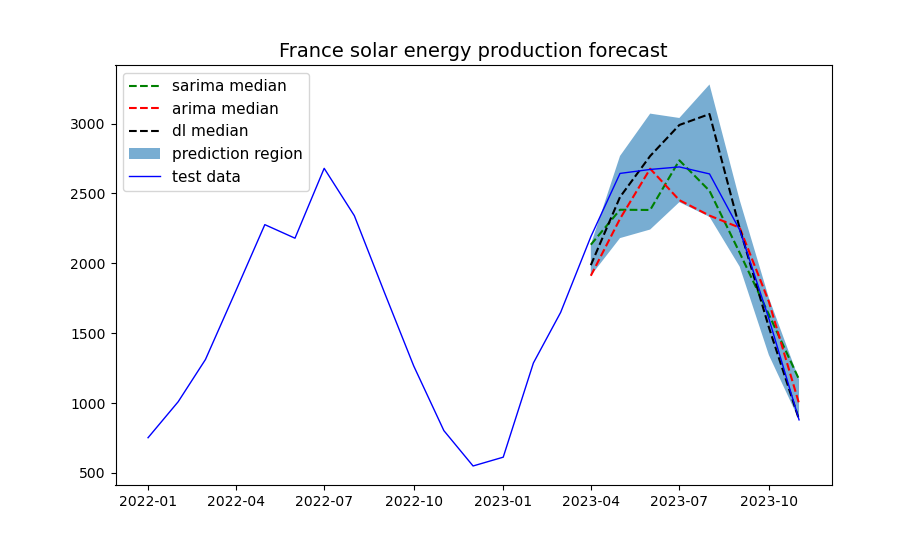
\includegraphics[width=0.4\textwidth]{figures/Figure_1.png}
    \caption{France solar energy production forecast}
    \label{fig:solar_forecast} % Tag for referencing
\end{figure}

Figure (~\ref{fig:solar_forecast}) visualizes the forecasts of solar energy production in France against the real values. From the visual analysis, both models perform quite well with some months more accureately forecasted through ARIMA model, and most of the forecasting results exhibit similar pattern. \\



\section{Conclusion}

\section{References}

\end{document}

